\documentclass[../Master.tex]{subfiles}
\begin{document}
\chapter{Introduction}
\section{Supramolecular Chemistry, why?}\label{sec:supramolecular-chemistry}
Supramolecular chemistry can be classified as the branch of chemistry concerned about the interplay between designed molecular assemblies and intermolecular bonds, or more colloquially referred to as ``chemistry beyond the molecule''\cite{desiraju_chemistry_2001}. \\
The discipline focuses on the design and synthesis of molecular architectures by relying on the complementary recognition, and subsequent assembly, of well-defined subunits. The products of complementary synthesis, the so-called ``supermolecules'' are sustained by non-covalent interactions such as hydrogen bonding, halogen bonding, coordination forces and \(\pi-\pi\) interactions. \\
The emergence of supramolecular chemistry has directly influenced how efficiently chemists can design and synthesize desired frameworks. The development and application of the bottom up approach is widely successful, owing to the non-covalent forces that dictate structural and morphological properties, while producing structures that were previously inaccessible.

\subsection{Host-Guest Chemistry}\label{subsec:host-guest-chemistry}
In supramolecular chemistry, host–guest chemistry describes complexes that are composed of two or more molecules or ions that are held together in unique structural relationships by forces other than those of full covalent bonds. Host–guest chemistry encompasses the idea of molecular recognition and interactions through non-covalent bonding. Non-covalent bonding is critical in maintaining the 3D structure of large molecules.\\
Host-guest interaction has raised dramatic attention since it was discovered. It is an important field because many biological processes require the host-guest interaction, and it can be useful in material designs.

\subsection{Metal-Organic Frameworks}\label{subsec:mof}
Metal-Organic Frameworks represent since 1995 \cite{yaghi_hydrothermal_1995} an exciting and rapidly growing area of research within the field of supramolecular chemistry.\\
MOFs' chemistry is a specific type of supramolecular chemistry that involve the coordination of metal ions with organic ligands to form highly porous and crystalline materials with a unique structure. \\
MOFs are obtained from the reaction between an organic linker and inorganic species, such as clusters or metal ions. The metal ions act as nodes that are connected by the organic ligands to create a three-dimensional framework. By understanding and tweaking the features of this two components within the material, it is possible to predict and tune the chemical and physical properties of the framework.\\
This offers a wide range of tunable properties that depend both from the inorganic joints and the organic linkers. By looking closer at the organic linker, it is possible to imagine a tuning of the shape (e.g.\ ligand coordination angles), size (e.g.\ dimension of the ligand as expansion or shrink-age) but also, functionality (e.g.\ decoration of the pores depending on the sub-stituent of the organic unit) of the MOF.\\
The self assembly of these components, typically done in solution, generate a linkage extended in a 3D crystalline framework that is characterized by large pores filled of solvent. Interesting, this rigid structure can stand vacuum: after removal of the solvent molecules the structure usually remains intact. \\
The resulting structure has a large internal surface area and can adsorb gases and other molecules with high efficiency, making MOFs useful in a variety of applications, such as gas storage, catalysis, drug delivery and molecule harvesting.

\subsection{Carboxylate–Based Metal–Organic Frameworks}\label{cb-mof}

Carboxylate ligands are tipically obtained from the acid-base reaction of a carboxilic acid with an appropriate base, their electronic structure determine the properties that follows. \\
\begin{figure}[h!]
	\centering
	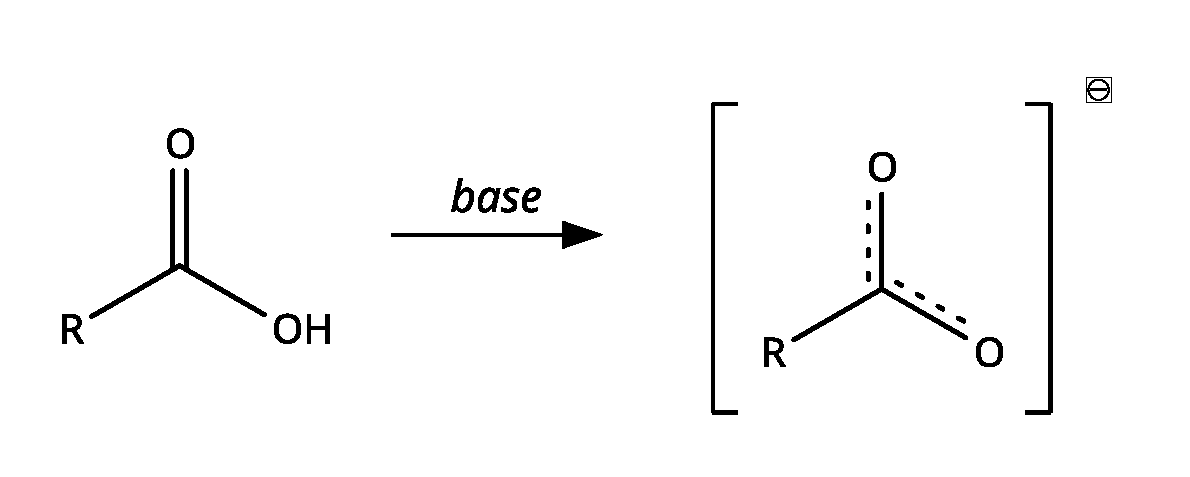
\includegraphics[width=10cm,height=3cm,keepaspectratio]{Structures/carboxstructure.eps}
	\caption{Carboxilate structure}\label{fig:carboxstructure}
\end{figure}

The carboxylate oxygen atoms can coordinate with metal ions through their lone pairs of electrons, forming metal-carboxylate coordination bonds. The metal-carboxylate bonds formed by carboxylate ligands are generally strong due to the high electronegativity of oxygen and the polarizability of the carboxylate group. The binding strength can be influenced by the nature of the metal ion, the electronic properties of the ligand, and the coordination geometry. Strong metal-carboxylate bonds contribute to the stability of the MOF framework. \\
The carboxylate group that can serve in multiple coordination mode although the chelating coordination mode is typically adopted: the ligand coordinates to the metal ion through both oxygen atoms.\\

\begin{figure}[h!]
	\centering
	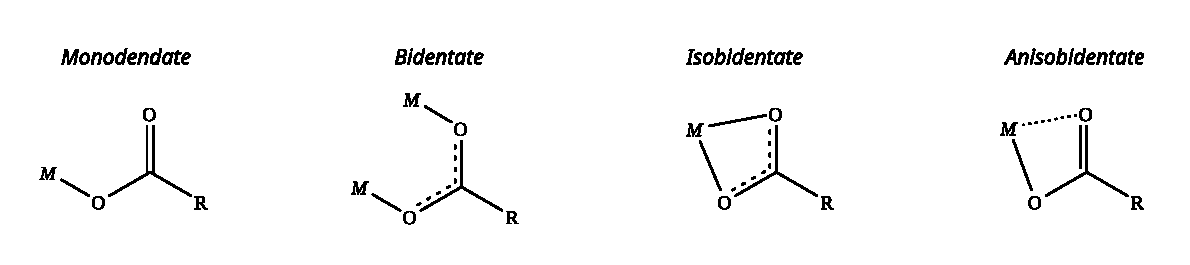
\includegraphics[width=16cm,height=3cm,keepaspectratio]{Structures/carboxcordmode.eps}
	\caption{Carboxilate coordination modes}\label{fig:carboxcordmode}
\end{figure}

Their geometric arrangement and flexibility can vary. The length and conformation of the carbon backbone connecting the carboxylate groups can affect the spatial arrangement of the ligand and rigidity or flexibility of the ligand can impact the packing arrangement and the resulting MOF structure. \\
Carboxylate ligands can also incorporate various functional groups, such as aromatic rings, electron-withdrawing or electron-donating groups, and functional moieties (e.g., -OH, -NH2). These functional groups can impart additional reactivity and chemical properties to the MOF, enabling specific applications. The presence of functional groups can also affect the hydrophobic or hydrophilic nature of the MOF.\\
The solubility of carboxylate ligands plays a crucial role in MOF synthesis. Some ligands are readily soluble in common solvents, facilitating the preparation of precursor solutions and the synthesis of MOFs. However, certain carboxylate ligands may exhibit limited solubility, necessitating the use of specialized solvent systems or modifications in reaction conditions to ensure proper ligand incorporation and MOF formation.

The divalent metal carboxylate based frameworks MOF-5 and HKUST-1 are examples of prototypical MOF materials and triggered a huge growth in the field of metal-organic frameworks.

\subsection{1,3–Diketones–Based Metal–Organic Frameworks}\label{dk-mof}
Classical \(\beta\)-diketones and related ligands have been studied for more than a century and their ability to give rise to a rich and interesting coordination and supramolecular chemistry is well documented\cite{aromi_poly_2008}. The widespread use of \(\beta\)-diketones structure as chelating ligand in coordination chemistry and the stability of its complexes with a number of metal ions originate from its chemical properties, determined by the keto–enol tautomerism.

\begin{figure}[h!]
	\centering
	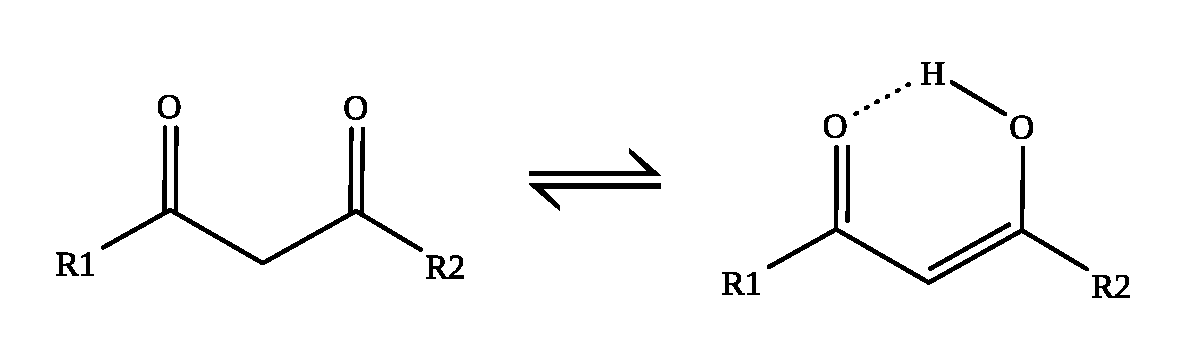
\includegraphics[width=10cm,height=3cm,keepaspectratio]{Structures/diktau.eps}
	\caption{\(\beta\)-diketones keto-entol tautomerism}\label{fig:diktau}
\end{figure}

\subsubsection{1,3-diketones as ligands}
They act under appropriate conditions as uninegative chelating donors, capable of stabilizing mononuclear or polynuclear complexes. One of the reason of such stabilization capability is the aromatic character of the chelate ring.
\begin{figure}[h]
	\centering
	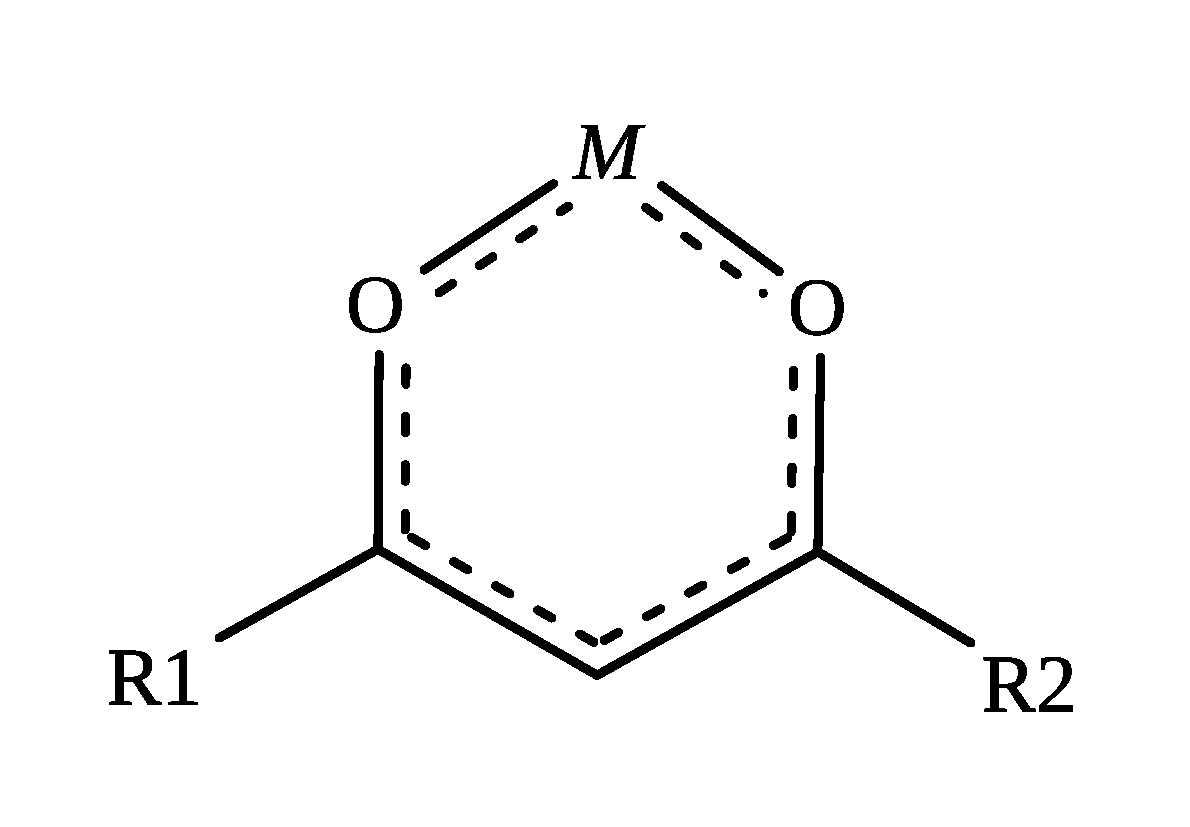
\includegraphics[width=10cm,height=3cm,keepaspectratio]{Structures/dikcordmode.eps}
	\caption{Coordination mode of $\beta$-diketones}\label{fig:diktaucordmode}
\end{figure}

\subsubsection{1,3-diketones MOFs examples}


\subsection{Azoles-Based Metal-Organic Framerworks}\label{az-mof}
Heterocycles are a remarkable class of compounds in terms of the biological, chemical and technological roles they play. Azoles, in particular, owe their importance to the fact that they occur in natural and synthetic molecules, but also to their fascinating coordinating chemistry, which has allowed their use in a wide range of applications. \\
Although azoles are mostly known as bases (i.e. pyridines), the five-membered azoles, including imidazole, pyrazole, triazole, and tetrazole can also be deprotonated to form the corresponding azolate anion. The possibility of generating this azolate anions not only it allows all N atoms to coordinate with metal ions in many different coordination modes, but also further increases the basicity of these donor sites. Consequently, azolate ligands can generate coordination compounds with a particularly high thermal and chemical stability  which is one of the most important issues for practical applications of coordination polymers.
For these reasones azolates have been widely used as bridging ligands for coordination polymers before the beginning of the past decade.
\subsubsection{Pyrazole Ring}
\begin{figure}[h]
	\centering
	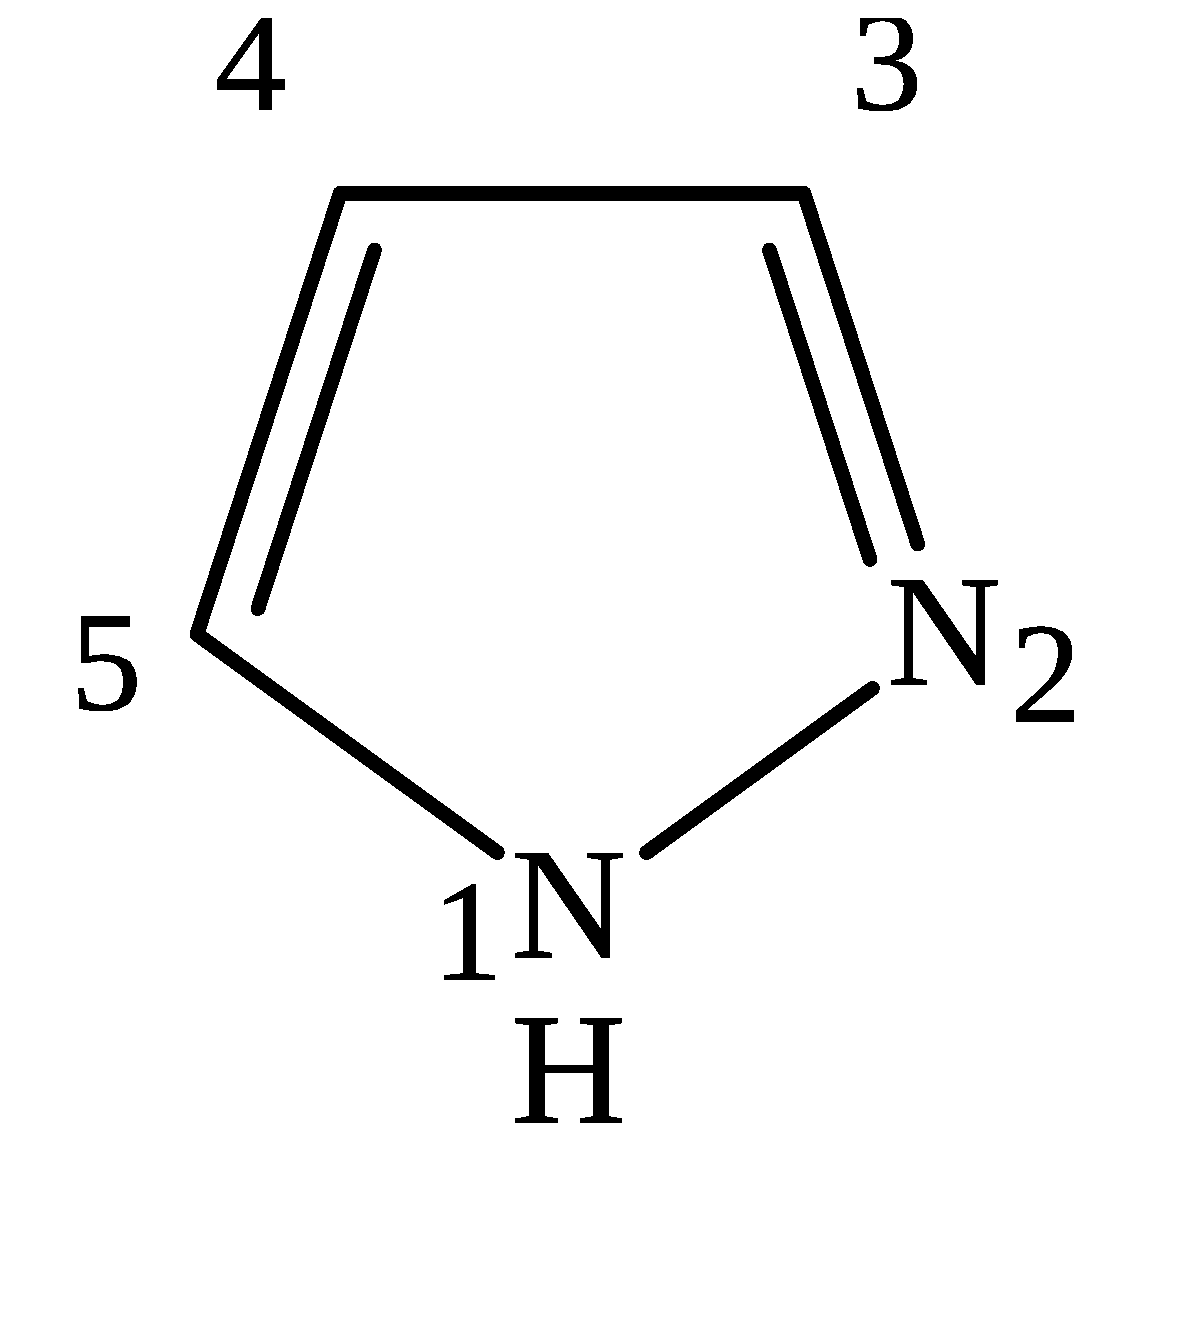
\includegraphics[width=6cm,height=3cm,keepaspectratio]{Structures/pyrazole.eps}
	\caption{Pyrazole structure}\label{fig:pyrstc}
\end{figure}
Simple 1H-pyrazoles have a Lewis acid N-H group at N$_1$ and a Lewis basic pyridine N-donor N$_2$ directly adjacent to each other. Thus, electronically, these heterocycles are both $\sigma$-donor and $\pi$-acceptor ligands. In addition, they are planar and non-bulky ligands. For these reasons, the pyrazole ring is one of the easiest and most flexible N-donor heterocycles to incorporate into larger polydentate ligand structures. \\
Pyrazole and only a handful of its derivatives are commercially available, but by using a variety of synthetic approaches it is possible to create substituted pyrazole rings with a wide range of substituents on their carbon atoms.
\subsubsection{Pyrazolate as ligands}
\begin{figure}[h]
	\centering
	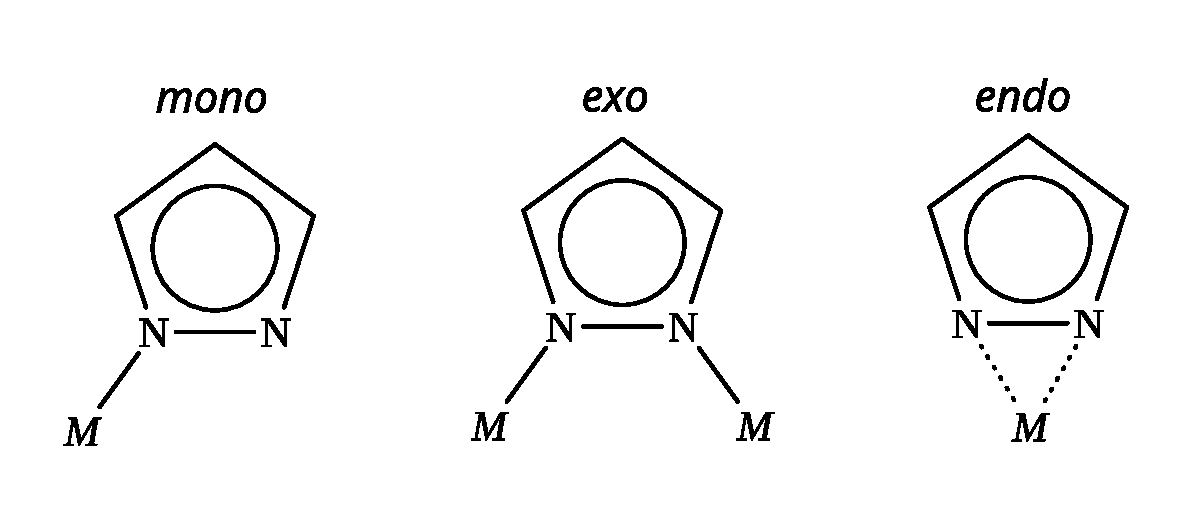
\includegraphics[width=10cm,height=6cm,keepaspectratio]{Structures/pyrazolecordmode.eps}
	\caption{Pyrazole coordination modes}\label{fig:pyrazole-cord-mode}
\end{figure}
Pyrazolate have been found to bind metals in a variety of coordination modes and can also act as bridging ligands.
After deprotonation of the N-H pyrazole, the obtained pyrazolate anion can be classified to act mainly in three different coordination modes:
\begin{itemize}
	\item  mono-dentate mode
	\item exo-bidentate \((\eta_{1}-\eta_{1})\)
	\item endo-bidentate \((\eta_{2})\)
\end{itemize}
This coordination ability is controlled by the nature of the metal ion and the substituents on the pyrazole ring, infact the substituents at the 3 and 5 positions (shown in \ref{fig:pyrstc} can modify the steric properties, whereas substituents at the 4-position can mainly change the electronic properties

\subsubsection{Pyrazolates MOFs examples}
MOF-303 and its derivates are an excellent example of pyrazole based MOFs with real applications as highly water-permeable and water harvesting capable materials.
They crystallizes in the monoclinic space group and its rodlike SBU consists of cis−trans-alternating corned-shared AlO6 octahedra.
\begin{figure}[h!]
	\centering
	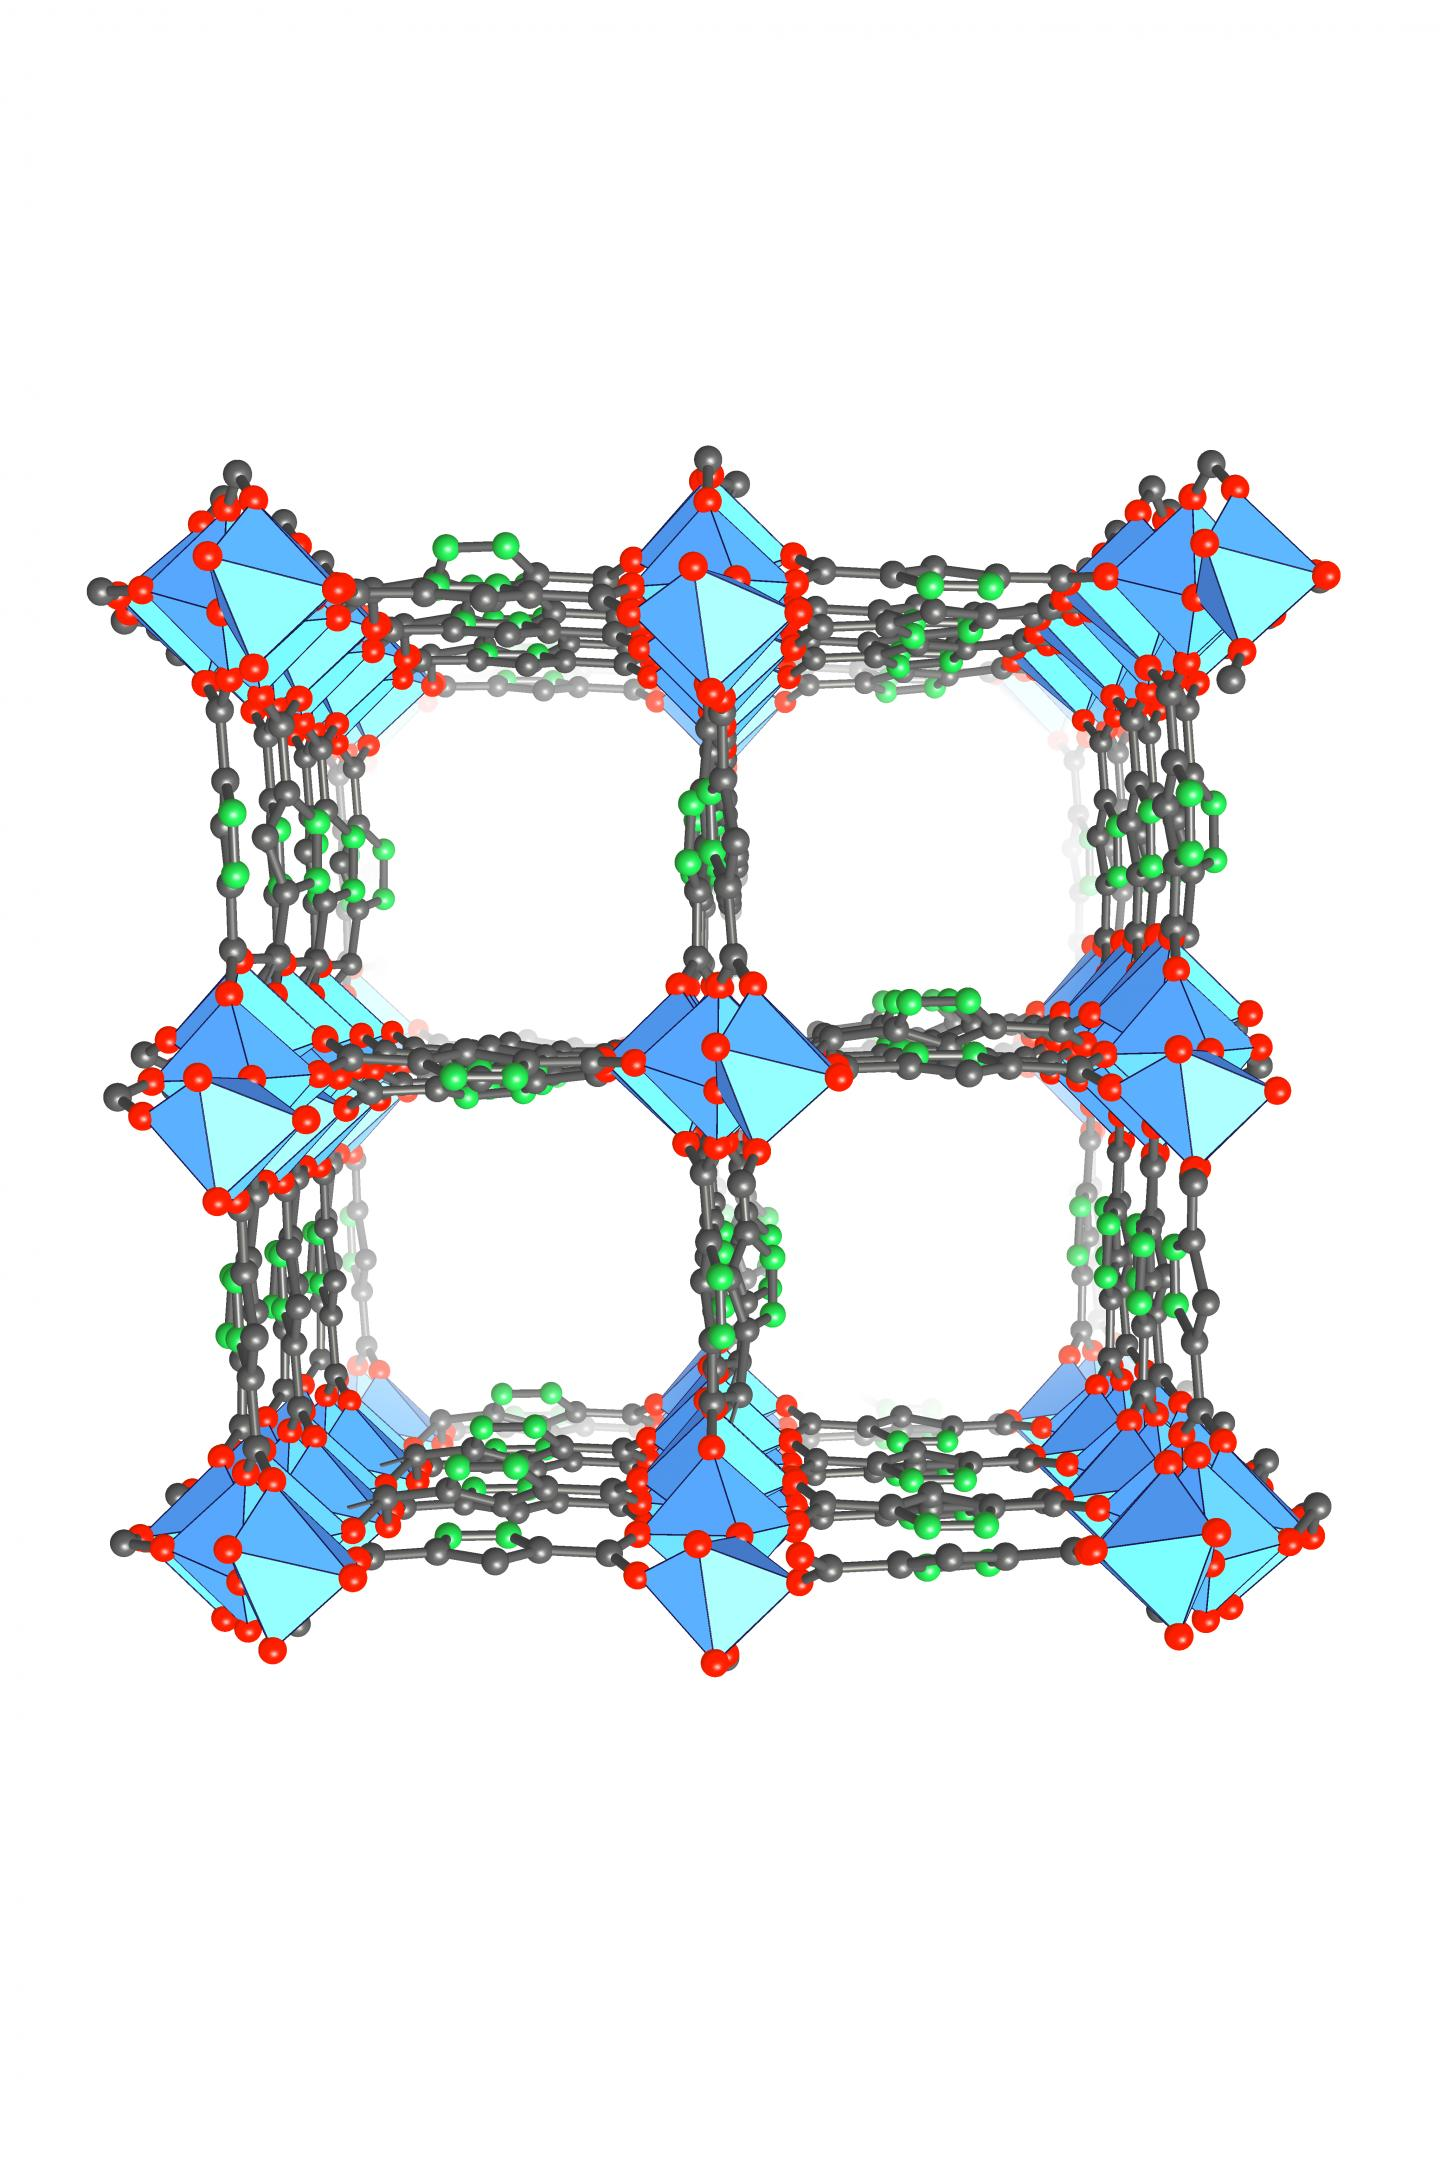
\includegraphics[width=6cm,keepaspectratio]{Images/MOF303.jpeg}
	\caption{MOF-303 structure}\label{fig:mof303structure}
\end{figure}
The

\end{document}
%%% Local Variables:
%%% mode: latex
%%% TeX-master: "../Master"
%%% End:

